\documentclass[letterpaper,11pt,twocolumn]{article}
\usepackage[T1]{fontenc}
\usepackage[utf8]{inputenc}
\usepackage{lmodern}
\usepackage{amsmath}
\usepackage{amsfonts}
\usepackage{amssymb}
\usepackage{amsthm}
\usepackage{float}
\usepackage{graphicx}
\usepackage{caption}
\usepackage{subcaption}
\usepackage{color}
\usepackage{xcolor}
\usepackage{url}
\usepackage{textcomp}
\usepackage{listings}
\usepackage{hyperref}
\usepackage{parskip}
\usepackage{todonotes}
\usepackage[
backend=biber,
style=alphabetic,
]{biblatex}
\usepackage{csquotes}
\setlength{\marginparwidth}{2cm}
\usepackage[inline]{enumitem}
\newlist{inlinelist}{enumerate*}{1}
\setlist[inlinelist]{label=(\roman*)}

\addbibresource{philo.bib}

\title{Behaviorism on AI}
\author{Paolo Marzolo}
\date{\today}

\begin{document}
\twocolumn[
    \begin{@twocolumnfalse}
        \maketitle
        %\tableofcontents
        \begin{abstract}
            The recent advancements in NLP have driven the field to asking fundamental questions on the degree of "understanding" of AI models. The (mostly) sudden ability of Large Language Models (LLMs) to analyze, manipulate and generate human-like text has resulted in the analysis of these AI models in mentalistic terms, considering themes like \textit{understanding, mind, reasoning}. This entails finding a definition for them in both the traditional, human sense and for the AI realm, increasing the scope of the original analysis. This article will propose Skinner's Behaviorism as a different doctrine under which analysis of such AI models is possible, highlight its strengths, consider how some of the more historically impactful criticisms of Behaviorism reflect on its use for AI, \textbf{and use it for comparisons between humans and AI behavior}.
        \end{abstract}
    \end{@twocolumnfalse}
    \medskip
]

\section*{Introduction}
Since the Artificial Intelligence research community shifted its main focus from symbolic to connectionist approaches, the difficulty of explaining the output of a model has grown to an entire field of study. In the eloquent words of one of the fathers of the field, \enquote{if
    you open them up and peer inside, all you can see is a big pile of goo}\cite{mozerUsingRelevanceReduce1989a}.
Many of the models which aim to describe and analyze human intelligence in various different fields, from expansive connectome maps\cite{yeSurveyCognitiveArchitectures2018a}, to advanced and biologically accurate neuron models of computational neuroscience, to detailed cognitive architectures\cite{yeSurveyCognitiveArchitectures2018a}, have grown at least as complex. Due to this, comparisons between the two generally go one of two ways:
\begin{description}
    \item[Shallow performance] Most AI benchmarks are set against human performance. Although benchmarks can be a fair way to evaluate performance, they do not allow for descriptive or predictive analysis: to do so requires an overarching theory in which benchmarks are inserted.
    \item[Reasoning and rationality] The other approach is often taken implicitly: on the human side, committing to an unspecified "general" cognitive theory; on the AI side, reading output as evidence for or against the AI's rightful belonging to the same cognitive theory. When dealing with language data in particular, when saying
        \enquote{One can see that GPT-4 easily adapts to different styles and produce impressive outputs, indicating that it has a flexible and general understanding of the concepts involved}\cite{bubeckSparksArtificialGeneral2023},
        the author and reader agree on
        \begin{inlinelist}
            \item considering concepts in their own minds,
            \item interpreting GPT-4's output as evidence of the existence of a similar "concept",
            \item GPT-4's concept causing its output to be more or less accurate.
        \end{inlinelist}
\end{description}

One can see how difficult any investigation becomes, as any hypothesis needs to solve some of the oldest and hardest philosophical questions about intelligence, rationality and minds. To counter this, in this article we will briefly investigate the use of a different doctrine to explain learning, historically presented to analyze biological organisms, but extensible to artificial agents: Behaviorism. In the text, we will distinguish the human Behaviorism from the artificially adapted one using the neologism BehAIviorism.

\begin{flushright}
    One does not simply follow behaviorism.\\
    \textit{Nobody (2023)}
\end{flushright}

As any doctrine which lasts long enough, Behaviorism has grown to many different variants: even wikipedia mentions seven\cite{Behaviorism2023}, while a recent review identifies 8\cite{araibaCurrentDiversificationBehaviorism2020}. In this article, we will focus on Radical Behaviorism, developed and championed by B.F. Skinner and later adapted and adopted by many different scholars. We will outline the general features of Behaviorism in the next two paragraphs. We wish to highlight that \enquote{Behaviorism is not the science of human behavior; it is the philosophy of that science (page 1, line 1)}\cite{skinnerBehaviorism1976}. Such philosophy, still, is tied to the science of human behavior, so some forays into it will be necessary. Armed with our newfound perspective, we will analyze AI through the lens of BehAIviorism, sidestepping philosophical implications of considering \textit{minds} and \textit{understanding} as \textbf{causes} of behavior, and instead focusing on the functional relations between stimuli, behavior and consequence;
% the same analysis can be replicated on human participants, and the results are comparable under the same theory \footnote[1]{isn't that a cool idea??}.
%As Skinner points out in "About Behaviorism", 

\section*{Fundamental claims of Behaviorism}
The Stanford Encyclopedia of Philosophy \cite{grahamBehaviorism2023} identifies three sets of claims. In this section, we analyze them in turn and consider what they would mean for AI analysis.
The first claim identifies behavior as the sole subject of psychology:
\begin{displayquote}
    Psychology is the science of behavior. Psychology is not the science of the inner mind - as something other or different from behavior.
\end{displayquote}
When applied to AI, this claim clarifies the boundaries of BehAIviorism: BehAIviorism investigates the relations between an AI agent's dataset and output, not the intricate calculations that created it.\footnote[2]{We stress that this claim does not consider genetic predisposition, but focuses on the distinction between behaviors and mental processes that generate it} As such, it distinguishes Machine Learning from BehAIviorism: while the first is a field \enquote{concerned with the question of how to construct computer programs that automatically improve with experience}\cite{mitchellMachineLearning1997}, the second will aim at framing AI agents' behavior inside a theory that can be used for both AI behavior and human behavior. \todo{this goes outside what behaviorism (as i explained) is and into behavior science!}


The second set of claims clarifies that the explanations of behaviors are to be sought
\enquote{without making ultimate reference to mental events or to internal psychological processes}.
This ultimate reference must instead reside in its functional \enquote{relation to or co-variation with the environment and to the animal's history of environmental interaction}. Just as in biological beings, the brain and its neurophysiological conditions implement these relations, so will gradient descent, self-attention and convolutional layers work to implement similar relations. And in the same way, they will not be causes themselves of the behavior of the agent.

Lastly, the third set extends the fundamental need for external, environmental causes to the terminology used, avoiding mental terms or concepts, either eliminating them or translating them into behavioral concepts. This would require a radical change in terminology, as the current literature (as the Sparks of AGI \cite{bubeckSparksArtificialGeneral2023} extract showed) leans quite heavily into mental terms as part of a "shared understanding" with the reader: an increase in the formality of the language would entail a loss of intuitive understanding by scholars not familiar with the terminology. A similar issue exists in Behaviorism circles: as an example, consider \href{https://abatechnologies.com/blog/behavior-analysiss-not-so-secret-agent}{this} blog post\cite{lattalBehaviorAnalysisNotSoSecret2020}, where the author offers a proposal to \enquote{say the same thing but without implying the participant is the agent of his or her choices}.

\todo[inline]{what now? initially i thought that it would make sense to continue with an overview of Behavior Science, then consider how Skinner models verbal behavior and from there draw comparisons with how it's taught to LLMs (spoiler: when you have direct access to the calculation done to decide what the next word should be you do it differently). But now I feel like that would mean going beyond "a version of behaviorism (the philosophy) would be useful to the CS world" and into some other, less defined thesis}

\section*{Behaviorism terminology and AI}
In this section, we will overview some basic elements shared between Behaviorism and Behavioral Science and review their BehAIvioristic counterpart. Let us remember that Behaviorism has a 70-year history\cite{schneiderHistoryTermRadical1987}, during which its characteristics were revised, reconsidered, extended and reworked: this can only be an introductory review.
\begin{description}
    \item[classical conditioning] test text
    \item[operant conditioning] test text
    \item[schedules of reinforcement] test text
\end{description}

To start this, we will need to define the terms we need to use

\section*{Verbal Behavior}
This section will first explain verbal behavior in behaviorism then highlight its similarities with RLHF

\subsection*{Speech and Behaviorism}

\subsection*{Training a LLM}


\section*{Criticisms and limitations}

\begin{description}
    \item[Chomsky and his long sneaky fingers like an aye aye]
        \begin{figure}[H]
            \centering
            \begin{subfigure}{.4\linewidth}
                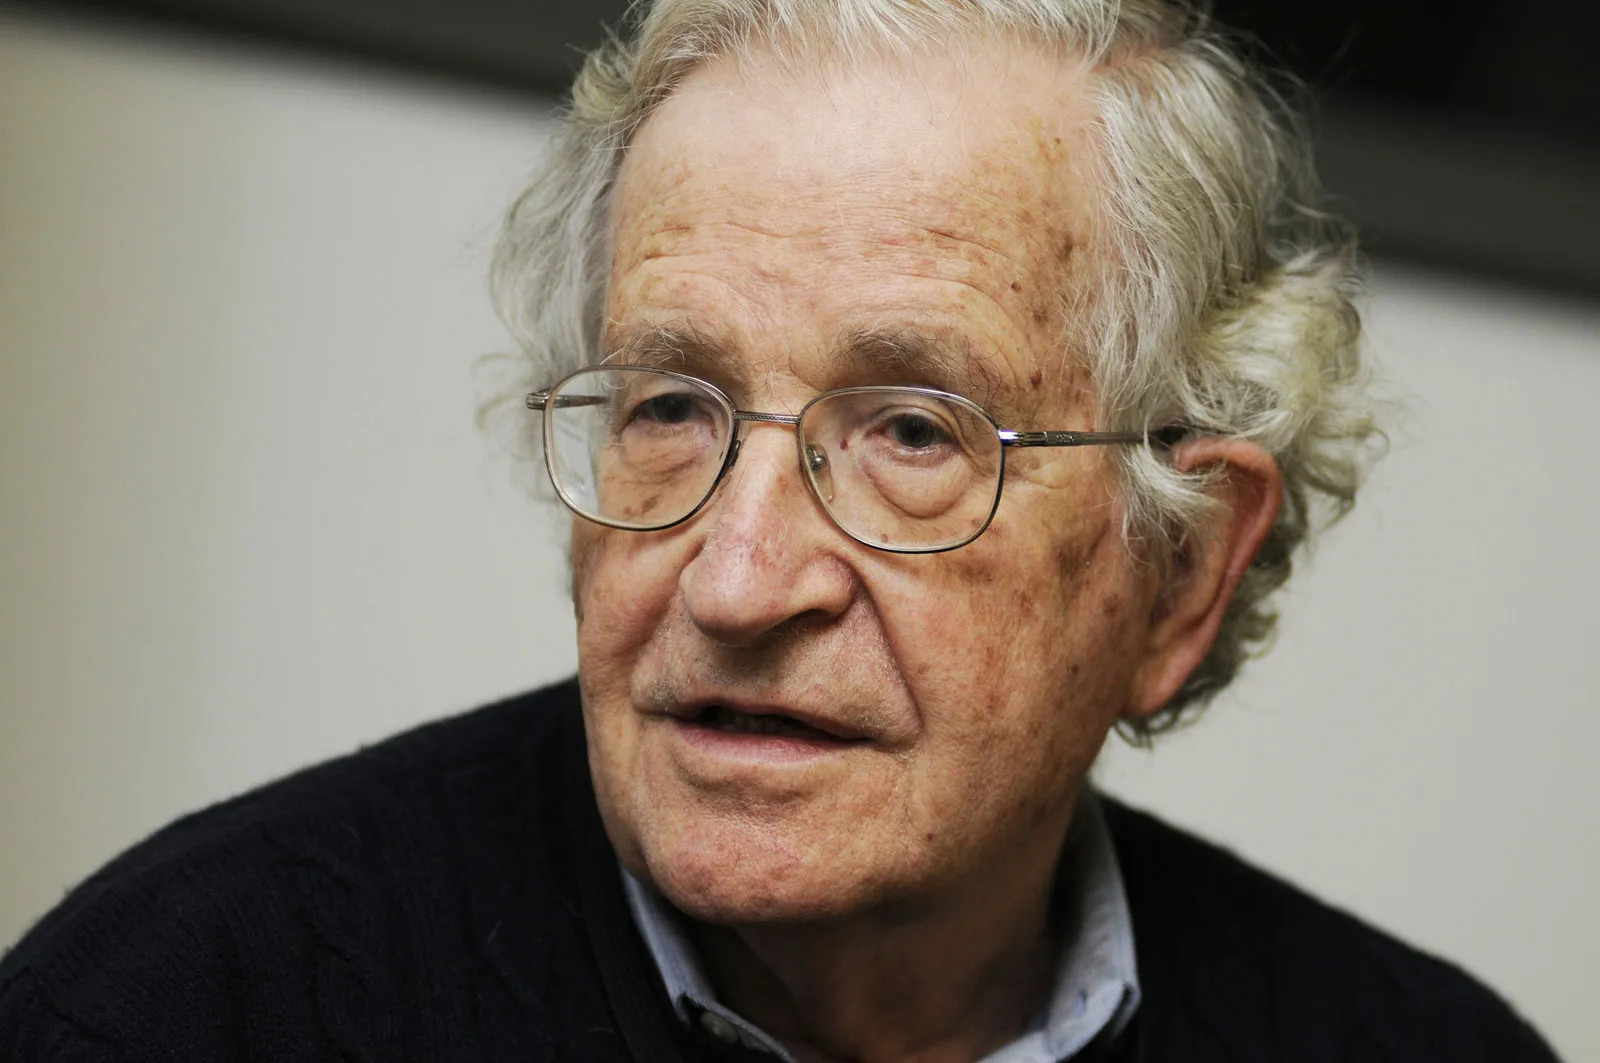
\includegraphics[width=\textwidth]{img/chomsky.jpeg}
            \end{subfigure}
            \begin{subfigure}{.4\linewidth}
                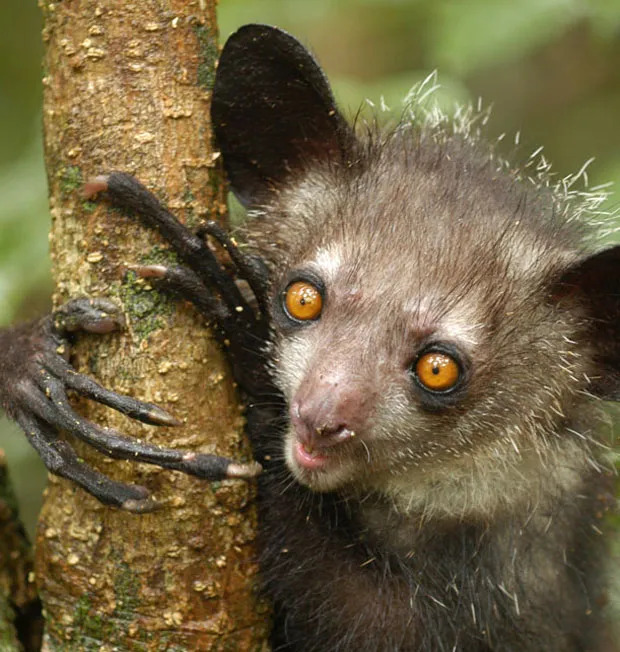
\includegraphics[width=\textwidth]{img/ayeaye.jpeg}
            \end{subfigure}
            \caption{a startling similarity.}
        \end{figure}

    \item[Different language means less intuition]
    \item[Why should machine intelligence follow behaviorism?]
    \item[But you can just program a rule]
\end{description}
is behaviorism an expressive enough framework to describe and predict AI agents' results?
to verify it, first we need to show how the basic terminology applies to AI agents. then, we will use the rich history of criticisms that have been raised against the discipline to battle-test our "implementation" of behaviorism. finally, we review why: to avoid mentalistic explanations of behavior and to have a "middle-ground theory" under which comparisons between results are fair...er.

\printbibliography


\end{document}